\section{Durchführung}
\label{sec:Durchführung}
Zunächst ist das Magnetfeld einer langen und einer kurzen Spule zu vermessen.
Der grundsätzliche Aufbau ist in Abbildung \ref{fig:Aufbau_langekurzespule} zu sehen.
\begin{figure}
  \centering
  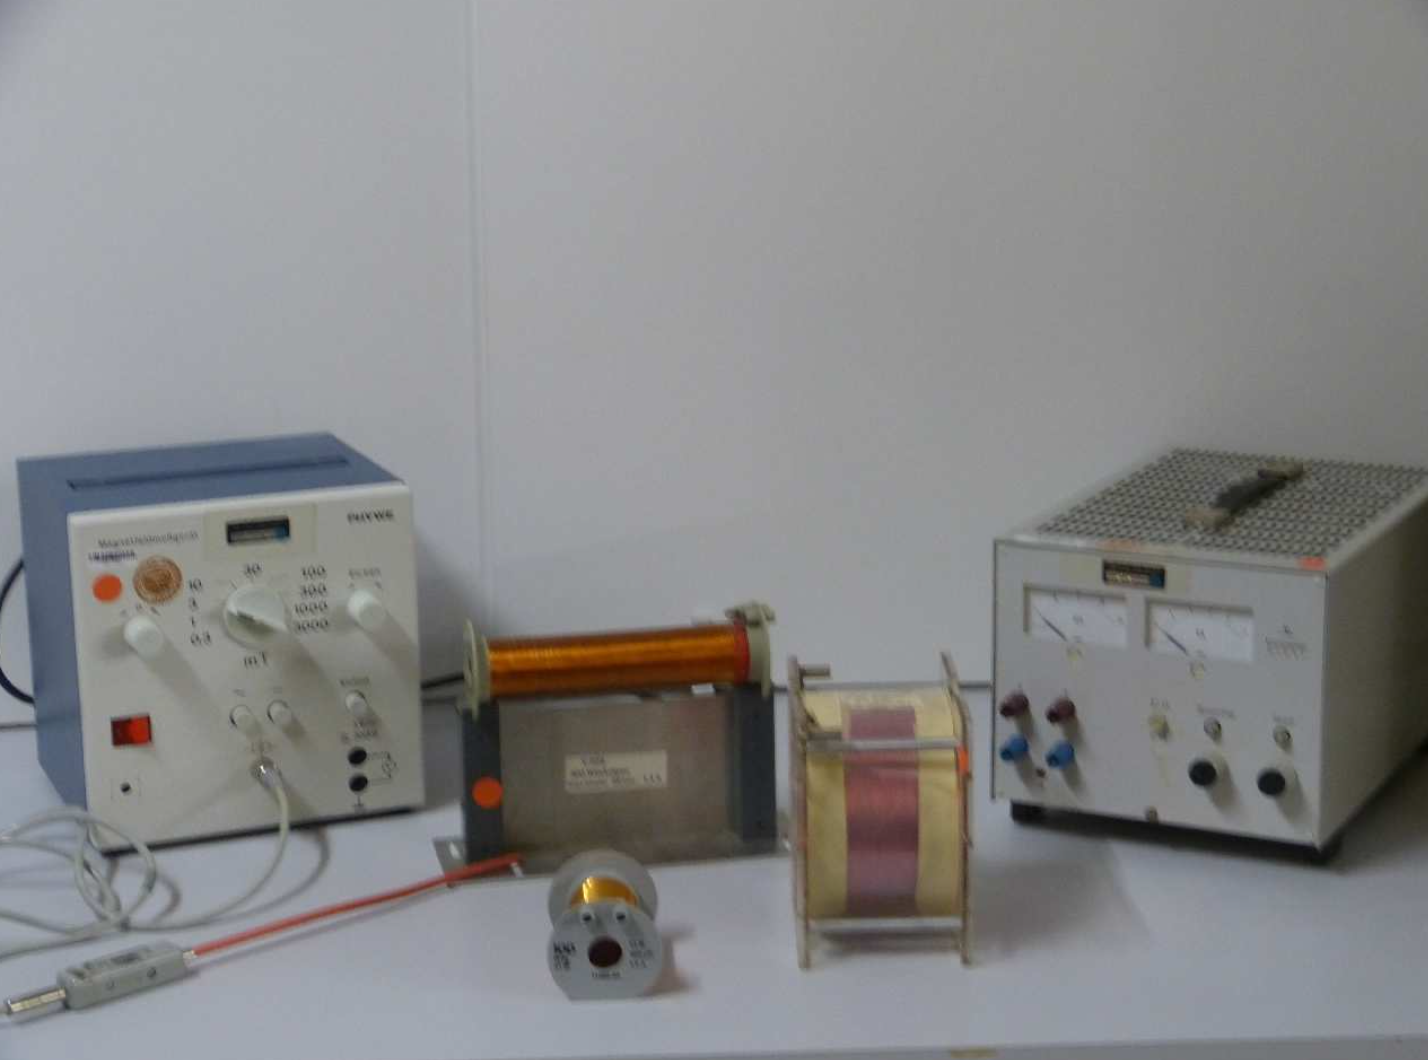
\includegraphics[width=300pt]{data/aufbau1.png}
  \caption{Aufbau zur Vermessung des magnetischen Feldes einer
  langen und einer kurzen Spule \cite{Versuchsanleitung}}
  \label{fig:Aufbau_langekurzespule}
\end{figure}
Die stromdurchflossene Spule wird mit ihrer Achse parallel zu einem langen Lineal
aufgestellt. Eine Hall-Sonde ist an diesem Lineal in einer Einspannung befestigt und
auf ihm verschiebbar. Dadurch lässt sich das magnetische Feld in regelmäßigen Abstand
innerhalb und auf beiden Seiten außerhalb der Spule messen. Dabei ist zu beachten, dass
die Hall-Sonde möglichst mittig in der Spule ist, um das Feld möglichst nur auf
der Spulenachse zu messen. Dieses Verfahren wird sowohl für die lange als auch die kurze
Spule durchgefüht.

Danach wird das Magnetfeld eines Helmholtz-Spulenpaars gemessen. Die Versuchsanordnung
für diese Messaufgabe ist in Abbildung \ref{fig:Aufbau_helmholtz} zu sehen.
\begin{figure}
  \centering
  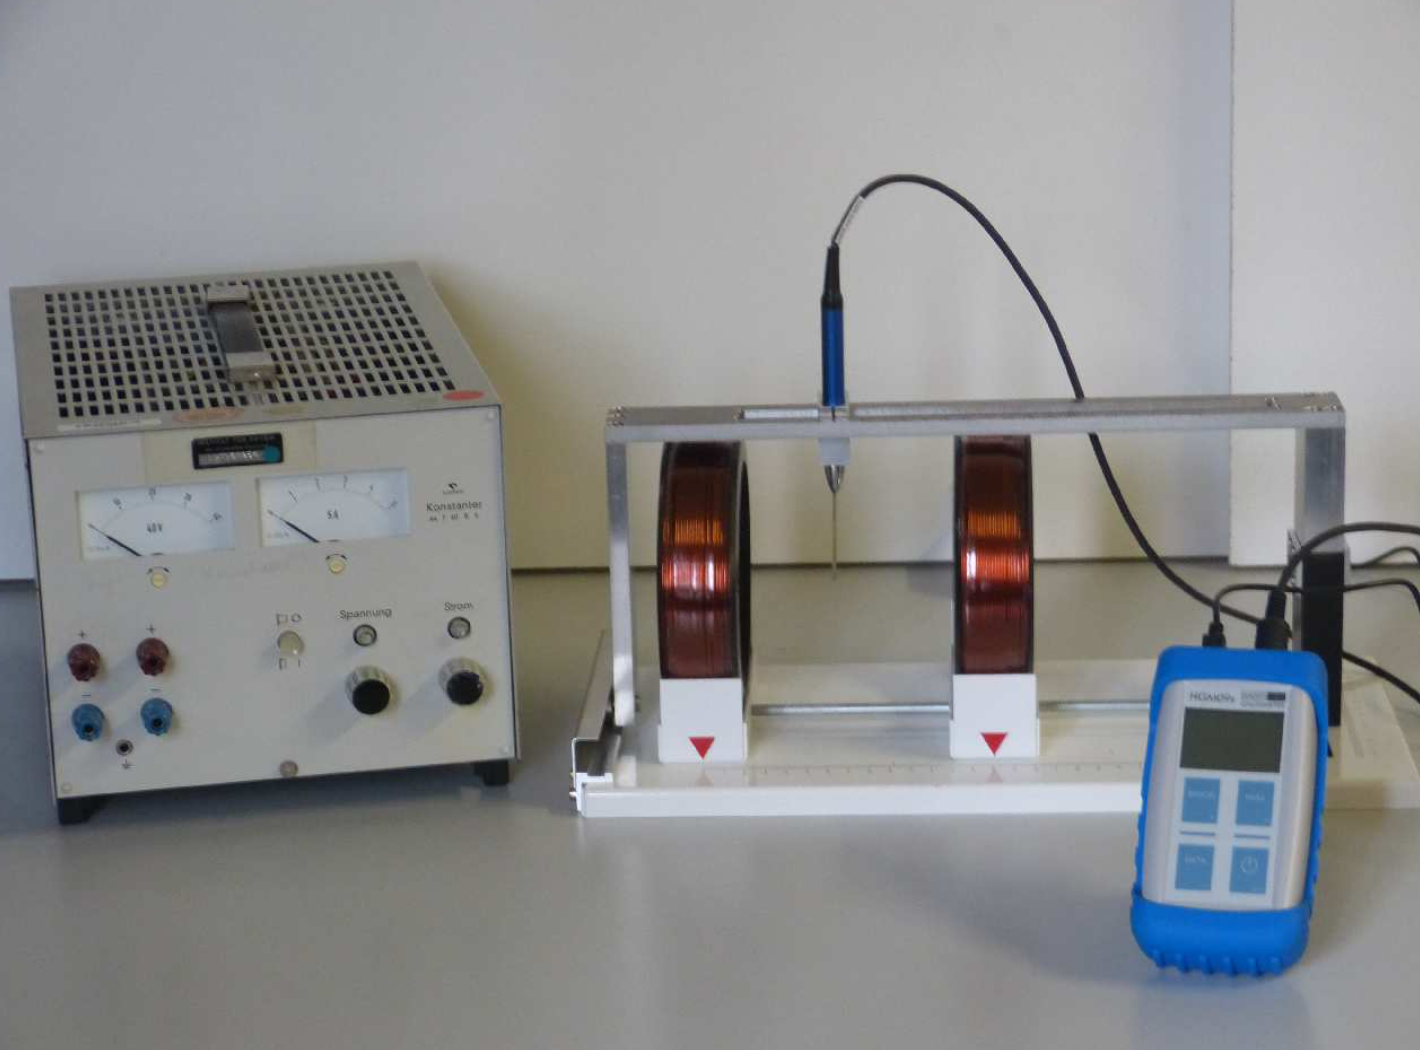
\includegraphics[width=300pt]{data/aufbau2.png}
  \caption{Aufbau zur Vermessung des magnetischen Feldes eines
  Helmholtzspulenpaars \cite{Versuchsanleitung}}
  \label{fig:Aufbau_helmholtz}
\end{figure}
Der Abstand der beiden Ringspulen wird mithilfe einer am Boden des Aufbaus
befindlichen Skala genau auf ihren Radius eingestellt. Sie werden mit einer Stromquelle
in Reihe geschaltet, um eine gleichsinnige Stromversorgung sicherzustellen.
Eine transversale Hall-Sonde ist auf der Symmetrieachse des Spulenpaars eingehängt und
dort frei verschiebbar. Mit ihr wird die magnetische Flussdichte entlang der Achse
gemessen. Aufgrund der Ausdehnung der Spulen nach oben hin ist es nur möglich,
in einem Teil des Innen- und Außenbereichs zu messen. Dies ist auch an der Abbildung
des Aufbaus ersichtlich.

Die letzte Messaufgabe besteht aus der Messung des Magnetfeldes einer Toroidspule
in Abhängigkeit der angelegten Stromstärke.
